\documentclass[final,authoryear,5p,twocolumn]{elsarticle}

\usepackage[bitstream-charter]{mathdesign}
%% \usepackage[adobe-utopia]{mathdesign}
\usepackage[T1]{fontenc}

\usepackage{/home/sci/weiliu/haldefs}
\usepackage{textcomp}
\usepackage{color}
\usepackage[vlined,ruled]{algorithm2e}
\usepackage{rotating}
\usepackage{array}

%% \usepackage{graphicx}
%% \usepackage{subfig}
%% \usepackage{hyperref}
%% \usepackage{amsmath}
%% \usepackage{verbatim}

%% \usepackage{mdwlist}

%% \hypersetup{
%%     unicode=false,          % non-Latin characters in Acrobat’s bookmarks
%%     pdftoolbar=true,        % show Acrobat’s toolbar?
%%     pdfmenubar=true,        % show Acrobat’s menu?
%%     pdffitwindow=false,     % window fit to page when opened
%%     pdfstartview={FitH},    % fits the width of the page to the window
%%     pdftitle={Hierarchical MRF for fMRI Journal draft},
%%     pdfauthor={Wei Liu},     % author
%%     pdfsubject={Functional Connectivity with fMRI},   % subject of the document
%%     pdfcreator={Wei Liu},   % creator of the document
%%     pdfproducer={Wei Liu}, % producer of the document
%%     pdfkeywords={functional MRI, connectivity}, % list of keywords
%%     pdfnewwindow=true,      % links in new window
%%     colorlinks= true,       % false: boxed links; true: colored links
%%     linkcolor=red,          % color of internal links
%%     citecolor=blue,        % color of links to bibliography
%%     filecolor=magenta,      % color of file links
%%     urlcolor=cyan           % color of external links
%% }

\begin{document}

\begin{frontmatter}
  \title{Multi-Level Functional Connectivity by Markov Random Field}

  \author[sci]{Wei Liu}
  \ead{weiilbu@sci.utah.edu}

  \author[sci]{Suyash P. Awate}
  \ead{suyash@sci.utah.edu}

  \author[sci]{P. Thomas Fletcher}
  \ead{fletcher@sci.utah.edu}

  \address[sci]{Scientific Computing and Imaging Institute, University of
  Utah, USA}

  \begin{abstract}
    Identifying functional networks from resting-state functional MRI is a
    challenging task, especially for multiple subjects. Most current studies
    estimate the networks in a sequential approach, i.e., they identify each
    individual subject's network independently to other subjects, and then estimate
    the group network from the subjects networks. This one-way flow of information
    prevents one subject's network estimation benefiting from other subjects. We
    propose a hierarchical Markov Random Field model, which takes into account both
    the within-subject spatial coherence and between-subject consistency of the
    network label map. Both population and subject network maps are estimated
    simultaneously using a Gibbs sampling approach in a Monte Carlo Expectation
    Maximization framework. We compare our approach to two alternative groupwise
    fMRI clustering methods, based on K-means and Normalized Cuts, using both
    synthetic and real fMRI data. We show that our method is able to estimate more
    consistent subject label maps, as well as a stable group label map.
  \end{abstract}

  \begin{keyword}
    resting-state functional MRI, segmentation, functional connectivity
  \end{keyword}
\end{frontmatter}

\section{Introduction}
Resting-state functional MRI (rs-fMRI) is widely used for detecting the
intrinsic functional networks of the human brain. The analysis of rs-fMRI data
is a challenging task, due to the scanner and physiological noise, head motion,
and subject's random thoughts during data acquisition. The availability of large
rs-fMRI databases open the door for systematic group studies of functional
connectivity. Despite that the inherent noise in rs-fMRI poses difficulty of
functional network estimation at the individual level, combining many subjects'
data together and jointly estimating the common functional networks is more
robust.

For identifying functional networks by using rs-fMRI of a single subject, One of
the most common approaches is independent component analysis (ICA) and its
variants \cite{calhoun2001spatial}. ICA recover the statistically independent
functional networks without \emph{a priori} knowledge of the regions of
interest. The functional networks can also be identified by solving an image
segmentation problem. By using clustering algorithms (also know as
parcellations), the brain voxels are partitioned into disjoint regions that
represent the functional networks.

As for study of multiple subjects, Group ICA \cite{calhoun2001spatial} is a
generalization of single-subject ICA. in group ICA, all subjects are assumed to
share a common spatial component map but have distinct time courses. The time
courses from all subjects are concatenated temporally, followed by a single
subject ICA. The subject component maps are obtained by a back-reconstruction
procedure. Alternatively, to generalize single-subject clustering methods to
group study, the time courses of all subjects can be concatenated just like
group ICA, resulting in a single group segmentation. Or, segmentations are
estimated from each single subject, and then are averaged to obtain a group
affinity matrix, based on which a second level segmentation is followed
\citep{bellec2010multi, van2008normalized}.

%% here is no explicit statistical modeling of the variability between the group
%% and subject component maps.  Ng et. al \cite{nggroup2012} use group
%% replicator dynamics to detect subject's sparse component maps, with group
%% information integrated into each subject's RD process.


%% Because the group level clustering is conducted after subject level clustering,
%% the clustering of one subject is unaware of the information from other subjects,
%% as well as the group clustering.

\begin{figure*}[htb]
  \centering
  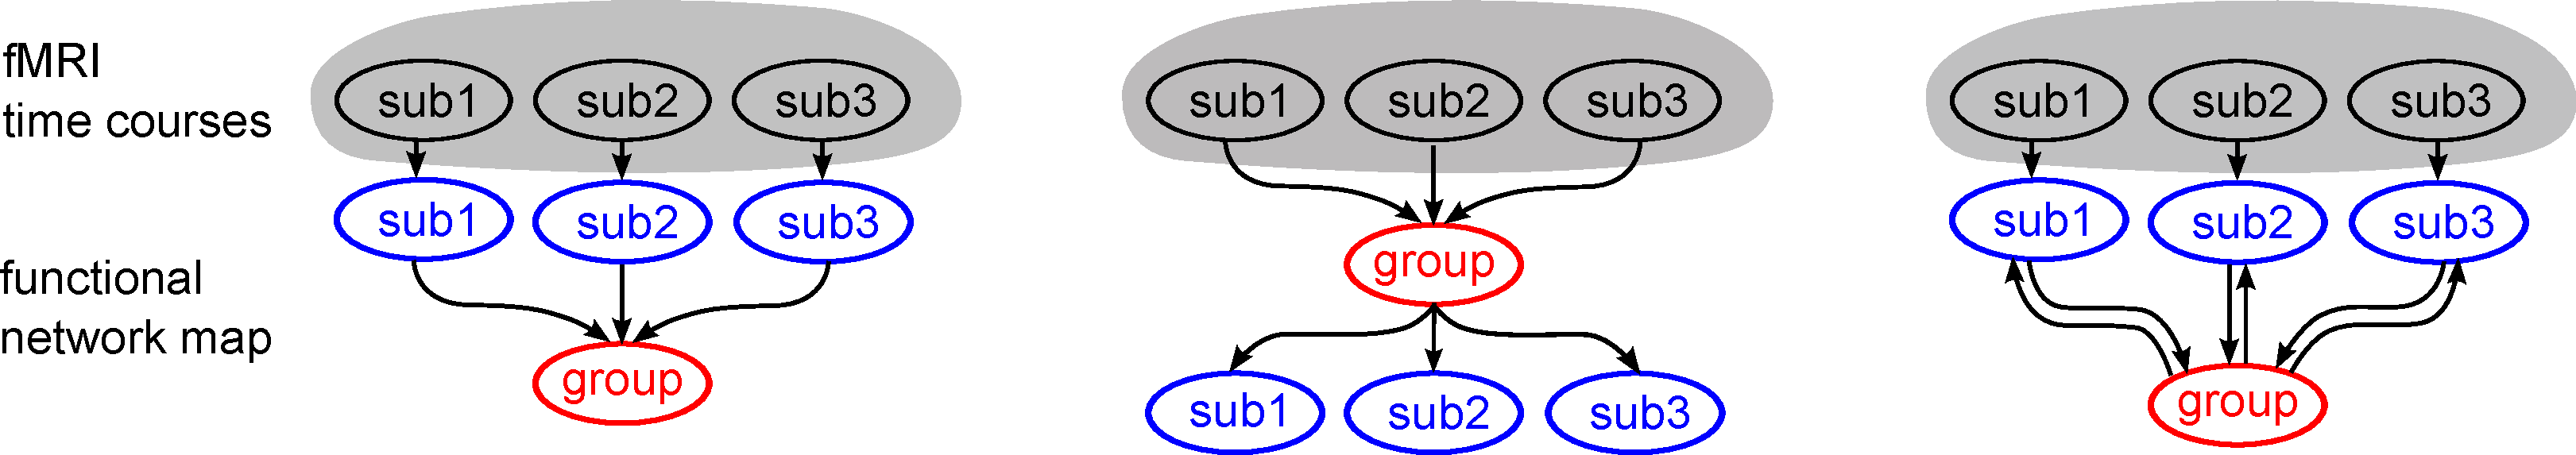
\includegraphics[width=0.9\textwidth]{figures/bidirections/bidirections}
  \caption{Comparison of segmentation methods for group study of fc-fMRI. Most
    methods are one-way approach, either in a bottom-up order in the left
    diagram, or the top-down order in the middle diagram. In left diagram, each
    subject's functional network map are estimated independent of other
    subjects, and a summary of the group's map is estimated from subject's
    map. In the middle diagram, a group map is obtained first, and it is used as
    a guide or a prior information for subject maps' estimation. Our methods aim
    at a joint estimation of both level of network maps, where group and
    subjects map help each other in a bidirectional flow, as show in the right
    diagram. }
  \label{fig:bidirections}
\end{figure*}

However, many of the currently used methods have one or more of the drawbacks
listed below:
\begin{itemize}
\item Due to the anatomical difference among subjects, the existing registration
  routines can not achieve perfect alignment. Hence even after project each
  subjects fMRI images into a common space, the time courses from different
  subjects may not map to same anatomical regions even they share same spatial
  coordinates. Together with the individual random thoughts during scan, these
  difference results in the inter-subject variability of the functional networks
  that must be modeled explicitly. Some methods~\citep{yeo2011organization} do
  not produce estimates of individual functional connectivity map. Such
  individual estimates are an important step in understanding functional
  networks not just on average, but also how these networks vary across
  individuals. Other methods such as the group ICA~\citep{ calhoun2001method,
    calhoun2001spatial}, does not have an explicit statistical model of the
  variability between the group and subject component maps. ((( we should add here that: spatial smoothing is often used for better matching between the subject's functional data)))

\item In the group analysis, subjects may exhibit similar but not exactly same
  spontaneous BOLD fluctuation. Current group studies typically first identify
  each subject's connectivity separately regardless of other subjects, and then
  estimate a \emph{pooled} summary of the group connectivity
  map~\citep{van2008normalized,craddock2011whole}. Or, a group map is estimated
  first, then is back-reconstructed to obtained the subject network
  map~\citep{calhoun2001method}. See figure \ref{fig:bidirections} for an
  illustration.  Such approaches are sub-optimal, since estimation of one
  subject's connectivity does not benefit from other subjects. From a Bayesian
  point of view, once the population distribution is known, it can help each
  subject's estimation as a prior. Subjects network estimates also gives
  feedback on group estimation.
\end{itemize}

We need a data-driven, unified probabilistic framework and put the connectivity
variables of both group and subjects jointly into this model. Inference can be
made from the posterior distribution of the variables in both (subject and
group) levels given the observed time series data.

In this paper we propose a Bayesian hierarchical model including both subject
and group levels in order to identify the functional networks from rs-fMRI data.
We assume a group network label map that acts as a prior to the label maps for
all subjects in the population. This Bayesian perspective provides a natural
regularization of the estimation problem of a single subject using information
from the entire population. The variability between the subjects and group are
taken into account through the conditional distributions between group and
subjects. The within-subject spatial coherence is modeled by a Markov Random
Field (MRF). [[ talk about the disadvantage of spatial smoothing, and our
    methods mitigate that.]]

[[Give a few examples of applications of MRF in neuroimaging, or give a one or
    two sentences of introduction for MRF.]] MRF is a statistical tool for
modeling the dependency of multiple hidden variables on a graph. Here we extend
the conventional concept of the spatial regularization with MRF by redefining
the graph including the network variables in the group and subject levels.

Furthermore, the full Bayesian model provides us an opportunity to study the
variability of the functional network by inference of the posterior. Besides the
traditional variance and confidence interval analysis, the mode of spatial
variability can be inferred from multivariate analysis. For the first time, to
our best knowledge, it would be possible to visualize how functional homogeneous
regions change along the principal direction of their posterior variability, and
compare these change across subjects.

[[Optimization of MRF. Past method, our method, exact optimization intractable,
    approximation]] Both the group clustering and subject clusterings are
estimated simultaneously with a Monte Carlo Expectation Maximization (MCEM)
algorithm. The model is data-driven in that all parameters, regularized by two
given hyper-parameters, are estimated from the data, and the only parameter that
must be specified is the number of networks.

[[ Talk about how the experiments is designed, both the synthetic data and real data. Test-retest data.]]

[[ talk about this is the extension of the preliminary results reported in miccai 2012. The difference: alternative formulation of the graphical model??? parameter estimation? ]]

[[ Our model is essentially a hidden Markov model with a carefully defined graph that represent the hierarchical structure of the group fMRI data. ]]


[[ Need a bullet list of the contribution of the paper ]]

[[ what does each section talk about in detail ]]

\section{Hierarchical Model for Functional Networks}
\label{sec:model}
We define each subject's network label map as a Markov Random Field (MRF) with
the neighborhood structure given by a regular lattice. The statistical
dependency between adjacent voxels acts as a prior model favoring spatial
coherence of functional regions. An additional group label map is defined on top
of all subject label maps. The group label map has the same Markov structure as
the individuals, again to encourage spatial coherence of the functional regions
in the group level. In addition, each voxel in the group map is connected to the
corresponding voxel in each subject. These connections model the relationship
between the group and the individuals. Hence, all voxels of subjects and group
label map are jointly connected into a single MRF. See
figure~\ref{fig:graphical} for an illustration.

More specifically, define a undirected graph $\mat G = (\mat V, \mat E)$. The
set of vertices $\mat V = (\mat V_G, \mat V_1, \cdots, \mat V_J)$ includes all
the voxels in the gray matter volumes $\mat V_j$ of all $J$ subjects as well as
those in the group volume $\mat V_G$.  An edge $(s, t) \in \mat E$ is defined if
1) $s\in \mat V_G, t\in \mat V_j$ and $s$, $t$ have the same physical
coordinates, or 2) $s, t\in \mat V_G$, and $s, t$ are spatial neighbors, or 3)
$s, t\in \mat V_j$, and $s, t$ are spatial neighbors. In our model we use
6-neighbor system in a 3D volume image. On each node $s \in \mat V$, a discrete
random variable $y_s \in \mat L = \{1,\cdots, L\}$ is defined to represent the
functional network labels.

\begin{figure}[htb]
  \centering
  \includegraphics[width=0.25\textwidth]{figures/graphical/grp2}
  \caption{Markov random filed is define on a graph that includes the voxels of
    all subjects as well as the group map. An edge is added when two voxels are
    spatial neighbors within one subject, or is added between two voxels if they
    are at different levels (that is, one in group map, the other in subject
    map), and share same physical coordinates. The square on subject level and
    time courses repeats the nodes in the square $J$ times, representing all the
    subjects nodes. For the cross-level connections, only the center voxels
    connection are shown, though the connections exist on all other voxels. }
  \label{fig:graphical}
\end{figure}

\subsection{MRF Prior} 
\label{sec:mrfprior}
MRF is a principal method for modeling the spatial context information. Here we
use it as a prior distribution of network label set $Y = \{y_s \in \mat L| s\in
\mat V \}$.  Our MRF prior on the hierarchical model is essentially a Potts
model \citep{potts1952some} with different weights on the within-subject
connections and the cross-level connections. Because of the equivalence of MRFs
and Gibbs fields~\citep{besag_spatial_1974}, we define the prior as $p(Y) =
\frac{1}{Z}\exp\{ -U(Y)\}$, where the energy function $U(Y)$ is given by the sum
of potential functions defined on the cliques:
\begin{align}
  U(Y) &= \sum_{s,r\in\mat V_G} \beta \psi(y_s, y_r) \nonumber\\
  &+ \sum_{j=1}^J \left ( \sum_{s\in\mat V_G, \tilde s\in\mat V_j} \alpha \psi(y_s, y_{\tilde s}) + \sum_{s,r\in\mat V_j}\beta\psi(y_s, y_r) \right ).\label{eq:energy}
\end{align}
Here $\psi$ is a binary function taking zero when the two inputs are equal and
one otherwise, and $\alpha$ and $\beta$ are parameters determining the strength
of the connections. $(s, r)$ is a pair of neighboring voxels at the same level
of the hierarchy (see figure \ref{fig:graphical}), and $(s, \tilde s)$ is a pair
of neighboring voxels at different level in the hierarchy, but share same
physical coordinates. However, according to our definition of the graph
including two levels, both $(s, r)$ and $(s, \tilde s)$ are neighbors, or,
cliques in the MRF, and can be treated equally in the following inference
procedure.

This regularization encodes two physiologically meaningful
\emph{a priori} assumptions on the functional networks under investigation: 1)
The networks are spatially coherent within single subject map and within group
map. This is modeled by the $\beta$ potential term . 2) The networks are similar
between subjects, and therefore between the group and subjects. This is modeled
by the $\alpha$ potential term.  The proposed energy function represents both
priors without introducing blurring artifacts.

[[need to add more advantage of the graph and the model]]

\subsection{Likelihood Model}
In the generative model, for any individual subject, the observed time course at
each voxel is assumed to be generated from a distribution conditioned on the
network label at that voxel. In fMRI analysis the time series at each voxel is
usually normalized to be zero mean and unit norm, so the analysis is robust to
shifts or scalings of the data. This results in the data being projected onto a
high-dimensional unit sphere. After normalization, the sample correlation
between two time series is equal to their inner product. Therefore the problem
of clustering voxels with high correlations can be reformulated to finding
clusters with small within-cluster distance on the sphere, where the distance is
defined by the inner product of two vectors.


We use $ X = \{ (x_1, \dots, x_N)\, |\, \ x_s \in S^{p-1} \}$ to denote the set
of \emph{normalized} time series on $p$-sphere. Given $Y$, the random vectors $
x_s$ are conditionally independent, hence $\log p( X | Y) = \sum_{s \in \mat V_j} \log
p (x_s | y_s)$.  The likelihood function $p( x_s | y_s)$ is naturally modeled by
a von Mises-Fisher (vMF) distribution
\begin{align}
 f ( x_s| y_s = l; \mu_l, \kappa_l) &= C_p(\kappa_l) \exp \left(\kappa_l  \mu_l^{\intercal} x_s\right), \label{eq:vmf}\\
  & x_s \in S^{p-1},  \quad  l \in {\mat L},  \nonumber
\end{align}
where for the network cluster label $l$, $\mu_l$ is the mean time course,
$\kappa_l \geq 0$ is the \emph{concentration parameter}, and $C_p$ is the
normalization constant. The larger the $\kappa_l$, the greater the density
concentrated around the mean. Since \eqref{eq:vmf} depends on $x$ only through
$\mu^T x$, the vMF distribution is unimodal and rotationally symmetric around
$\mu$.

\section{Bayesian Inference}
\label{sec:inference}
We solve the inference problem in a \emph{maximum a posteriori} (MAP)
framework. That is, given the observed time course data $X$, we estimate the
posterior mode of $p(Y|X)$. This consists of the following components.

\subsection{Parameter Estimation} 
In this data-driven model, we propose to estimate the parameters $\theta =
\{\alpha, \beta, \kappa, \mu\}$ from the data using an Expectation Maximization
(EM) algorithm. However, the high-dimensionality and dependency between
spatially adjacent voxels in MRF make it infeasible to obtain a closed form
solution of the expectation of $\log p(X,Y)$ with respect to $p(Y|X)$. Here we
propose to approximate the expectation using Monte Carlo EM (MCEM), in which a
set of samples, $(Y^1, \cdots, Y^M)$, generated from density $p(Y|X)$ is used to
approximate the expected value by the empirical average
$\frac{1}{M}\sum_{m=1}^M\log p (X, Y^m)$.

\subsection{Gibbs Sampling} 

[[ talk about conditional independency in order to introduce the Gibbs sampling ]]

Gibbs sampling converts a multivariate sampling problem into a consecutive
univariate sampling, hence is well adapted to draw the Monte Carlo samples from
$p(Y|X)$.  In our hierarchical structure, the sampling procedure is also done in
a multi-level fashion. At the image level, a sample of the group label map,
$Y^m_{G}$, is drawn given the previous subject label map, $Y^{m-1}_j$. Next, a
sample for each subject map, $Y^m_j$, is generated given the current group label
map, $Y^m_G$.  At the voxel level, we draw samples of the label $y_s$ given the
rest of nodes fixed, and update $y_s, \forall s \in V$. The conditional
probability used to generate samples at the group and subject voxels are given
as
\begin{align}
p(y_s | y_{-s},X) &\propto \frac{1}{Z_s}\exp\{-U(y_s | y_{-s})\} \cdot p(x_s | y_s) \\
&= \frac{1}{Z_s}\exp\{-U_p(y_s | y_{N(s)}, x_s)\} \nonumber\\
U_p &= \alpha\sum_{j=1}^J \psi(y_s, y_{\tilde s}^j) + \beta\sum_{r\in N(s)} \psi(y_s,y_r), \forall s \in \mat V_G, \label{eq:enggrp}\\
U_p &= \alpha \psi(y_s,y_{\tilde s}) + \beta\sum_{r\in N(s)} \psi (y_s, y_r) \nonumber \\
& - \kappa_l \mu_l^{\intercal} x_s - \log C_p, \: \forall s \in \mat V_j, \label{eq:engsub}
\end{align}
where $-s$ is the set of all nodes excluding $s$, $Z_s$ the normalization
constant, $U_p$ is the posterior energy, and $N(s)$ is the set of neighbors of
$s$.  $y_{\tilde s}^j$ in \eqref{eq:enggrp} is the network label of subject $j$'s voxel
with the same physical coordinates with $s$, and $y_{\tilde s}$ in
\eqref{eq:engsub} is the label of group's voxel with the same physical coordinates
with $s$. Because of the dependency on previous samples, the sequence of samples
will be a Markov Chain, hence our method falls into Markov Chian Monte Carlo
(MCMC) sampling.  After a sufficient burn-in period, a series of samples $Y^m, m
= 1\cdots M$ is saved for approximating the expectation $\mathbb{E}[\log
  p(X,Y)]$.

\subsection{Pseudo likelihood} 
To evaluate $\log p(X,Y^m;\theta) = \log p(Y^m;\theta) + \log p(X|Y^m;\theta)$
as a function of $\theta$, we face the difficulty of evaluating the partition
function $Z$ in $p(Y^m)$.  In practice the Gibbs field is approximated by
pseudo-likelihood~\citep{besag_spatial_1974}, which is defined as the product of the conditional
distribution $p(y_s|y_{-s}), \forall s \in \mat V$. Therefore the energy
function can be written as
\begin{align*}
U(Y) &\approx  \sum_{s\in\mat V} U(y_s | y_{-s}) \\
&= \sum_{s\in\mat V_G} \left ( \alpha \sum_{j=1}^J \psi(y_s,y_{\tilde s}^j) +\beta\sum_{r\in N(s)} \psi(y_s, y_r) \right ) \\
&+ \sum_{j=1}^J \sum_{s\in\mat V_j} \left (\alpha \psi(y_s, y_{\tilde s}) + \beta \sum_{r\in N(s)} \psi(y_s, y_r) \right ),
\end{align*}
where $y_{\tilde s}^j$ and $y_{\tilde s}$ has the same definition with \eqref{eq:enggrp} and \eqref{eq:engsub}.

\subsection{Hierarchical MRF algorithm using MCEM} 
With all the preparation above, parameter estimation can be done by maximizing
$\frac{1}{M}\sum_{m=1}^M\log p (X, Y^m)$. The $\alpha$ and $\beta$ in the MRF
prior can be optimized by maximizing $\frac{1}{M}\sum_{m=1}^M\log p (Y^m)$ with
a Newton-Raphson method. We assume a Gaussian prior distribution on $\alpha$
with hyper-parameters $\mu_{\alpha}$ and $\sigma_{\alpha}$, which is given
manually and does not have significant impact on the model. In order for MCMC
sampling to converge quickly to the posterior, we need a reasonably good initial
network label map. Here the K-means clustering on a concatenated group dataset
is used for the initial maps of both the group and subjects. After the EM
parameter estimation iterations are done, an Iterated Conditional Modes (ICM) on
the current sample map gives the final label maps. Putting this all together,
the \textsf{groupmrf} algorithm to estimate the group and individual label maps
is given in Algorithm \ref{alg:alg1}.

\begin{algorithm}
  %% \SetAlgoLined
  \KwData{Normalized fMRI, initial group label map}
  \KwResult{Group label map $Y_G$, subjects label map $Y_j, j\in\{1,\cdots, J\}$, parameters $\{\alpha, \beta, \mu, \sigma\}$}
  \While{$\mathbb{E}[\log p(X, Y)]$ not converge}{
    %% E step\;
    \Repeat{$B+M$ times}{
      \lForEach(){$s \in \mat V_G$}{
        Draw consecutive samples of $y_s$ from $p(y_s | y_{-s}, X;\theta)$ using \eqref{eq:enggrp}
      }
      \ForEach(){$j  = 1\dots J$}{
        \lForEach(){$s \in \mat V_j$}{
        Draw consecutive samples of $y_s$ from $p(y_s | y_{-s}, X; \theta)$ using \eqref{eq:engsub}
        }
      }
      Save sample $Y^m $ after $B$ burn-ins\;
    }
    %% M step\;
    \ForEach{$l = 1\cdots L$} {
      Estimate $\{\mu_l, \kappa_l\}$ by maximizing $\frac{1}{M}\sum_{m=1}^M\log p (X|Y^m)$\;
    }
    Estimate $\{\alpha, \beta\}$ by maximizing $\frac{1}{M}\sum_{m=1}^M\log p (Y^m)$\;
  }
  Run ICM on current samples to estimate final label maps.
  \caption{Monte Carlo EM for group MRF}
  \label{alg:alg1}
\end{algorithm}


\section{Experiments}
[[ This section should cover synthetic data, both 7 and 17 networks of real
    data?, bootstrap, posterior map. Do we want to split experiments and results
    in two sections? For now let me split them into two sections. ]] 

%% Since we have quite a few tests, have each test's experiments setup and
%% results in two sections seem cumbersome.  We may need put them in a single
%% section, with each subsection a specific test's setup and results. ]]

\subsection{Synthetic Data}
Since our \textsf{groupmrf} is an extension of existing clustering methods, we
compare our method with two other clustering method: \textsf{K-Means} and
normalized-cuts (\textsf{N-Cuts}), as well as two degenerated version of
\textsf{groupmrf} algorithm: the \textsf{groupmrf1} and \textsf{groupmrf2}.

%%  For experiments both on the synthetic and \emph{in vivo} data set, We apply
%% all three methods on the data and compare them.

The K-Means algorithm, as a simple and fast clustering method, was applied on
paradigm fMRI study in \citet{baumgartner1998quantification}, and later used by
\cite{bellec2010multi} for bootstrap analysis of a group of rs-fMRI. In our
experiment, the distance metric of \emph{K-Means} is defined as $1 -
x_s^\intercal x_r$.  we apply \textsf{K-Means} on each subject fMRI time courses
20 times, and choose one segmentation map with the minimal ratio of
inter-cluster sum-of-distance and intra-cluster sum-of-distance. For group
study, we obtain a \emph{group} dataset by concatenating all subjects time
courses. \textsf{K-Means} is applied 20 times on this group dataset again to
obtain a group network label map. the initial cluster centers for both subject
and group \textsf{K-Means} are chosen randomly but maximizing the between-center
distance~\citep{arthur2007k}.

Normalized cuts treats the fMRI image segmentation as a graph partitioning
problem, and propose a global criterion~\cite{shi2000normalized}.  It is used by
\citet{van2008normalized, craddock2011whole} for group rs-fMRI
study. following~\citet{van2008normalized}, we also apply \textsf{N-Cuts} in two
stages. First \textsf{N-Cuts} is run on each subject's affinity matrix, as
computed as the pairwise correlation between time courses. A second N-Cuts is
applied on a group affinity matrix, which is computed by summing up all of the
subjects' affinity matrix derived from their segmentation map. We use the
\textsf{Ncutclustering\_9} toolbox \cite{shi2000normalized}, a newer version of
the one used in \cite{van2008normalized}.

\begin{figure*}[htb]
\centering
  \begin{tabular}[]{ccccccc}
      & Truth & \textsf{K-Means} & \textsf{N-Cuts}  & \textsf{groupmrf1} & \textsf{groupmrf2} & \textsf{groupmrf}  \\
      \begin{sideways}group \end{sideways} &
      
\includegraphics[width=0.1\textwidth]{figures/syn/truth/grp} &
      
\includegraphics[width=0.1\textwidth]{figures/syn/smooth_kmeans/grp} &
      
\includegraphics[width=0.1\textwidth]{figures/syn/smooth_ncuts/grp} &
      
\includegraphics[width=0.1\textwidth]{figures/syn/smooth_groupmrf/grp} &
      
\includegraphics[width=0.1\textwidth]{figures/syn/na1} &
      
\includegraphics[width=0.1\textwidth]{figures/syn/nonsmooth_groupmrf/grp} \\

      \begin{sideways}sub 1 \end{sideways} &
      
\includegraphics[width=0.1\textwidth]{figures/syn/truth/sub01} &
      
\includegraphics[width=0.1\textwidth]{figures/syn/smooth_kmeans/sub01} &
      
\includegraphics[width=0.1\textwidth]{figures/syn/smooth_ncuts/sub01} &
      
\includegraphics[width=0.1\textwidth]{figures/syn/smooth_groupmrf/sub01} &
      
\includegraphics[width=0.1\textwidth]{figures/syn/nonsmooth_onelevel/sub01} &
      
\includegraphics[width=0.1\textwidth]{figures/syn/nonsmooth_groupmrf/sub01} \\

      \begin{sideways}sub 2 \end{sideways} &
      
\includegraphics[width=0.1\textwidth]{figures/syn/truth/sub02} &
      
\includegraphics[width=0.1\textwidth]{figures/syn/smooth_kmeans/sub02} &
      
\includegraphics[width=0.1\textwidth]{figures/syn/smooth_ncuts/sub02} &
      
\includegraphics[width=0.1\textwidth]{figures/syn/smooth_groupmrf/sub02} &
      
\includegraphics[width=0.1\textwidth]{figures/syn/nonsmooth_onelevel/sub02} &
      
\includegraphics[width=0.1\textwidth]{figures/syn/nonsmooth_groupmrf/sub02} 
  \end{tabular}
  \caption{Compare the group and subject network label maps estimated from the
    proposal \textsf{groupmrf} and other methods. Only two from all 25 subjects
    map are shown as a illustration. The simulated true maps, with regions of
    different sizes, and the average 90\% Rand index between group and subjects, well
    represent the functional network patterns in real data.}
  \label{fig:synmap}
\end{figure*}

\textsf{groupmrf1} is different with \textsf{groupmrf} in that it does not have
the within-subject and within-group links (i.e. the $\beta$ term in
\eqref{eq:energy}). \textsf{groupmrf2} is different with \textsf{groupmrf} in
that it does not have the between-level links (the $\alpha$ terms in
\eqref{eq:energy}). Hence \textsf{groupmrf2} amounts to define a MRF on each
single subject and estimate each subject's network label map indepedent of other
subjects. Such strategy is equivalent to the hidden Markov model we proposed in
\citet{liu2011monte}.  Both \textsf{groupmrf1} and \textsf{groupmrf2}, as
degenerated case of \textsf{groupmrf}, serve to check if a simplified model be
able to achieve same or better performance compared to the proposal model.

It is infeasible for our method, a clustering-based method to compare a
decomposition-based method, such as group ICA, since the former is more of a
disjoint partition and the later has overlapping membership assigned to each
voxel. However, a posterior map from our method will be shown for a qualitative
comparison with ICA component map.


We simulate synthetic rs-fMRI data in two steps: generating functional network
pattern maps, and generating time courses. Since we assume the network map a
MRF, we generate the group network map by random sampling a Potts model with
$\beta = 2.0$ and 500 scans. Given the group map, a subject map is generated
with $\alpha=0.5$ and $\beta = 2.0$ based on the definition of distribution in
equation \ref{eq:energy}. The subject map generation steps are repeated 25 times
to obtain 25 subjects in total. To simulate the time courses given the network
label map, we first generate mean time courses $\mu_l, l=\{1,\dots, L\}$ from a
first-order auto-regressive process $x_t = \varphi x_{t-1} + \varepsilon$ with
$\varphi = 0.8$ and noise variance $\sigma_{\varepsilon} = 0.1$. The sample
correlation between the mean time series is in the range of $(-0.15,
0.3)$. Then, independent Gaussian white noise of $\sigma^2 = 50$ are added on
each cluster's mean time course.


\section{Results}

\subsection{Synthetic Data}
The simulated true networks patterns map and the estimated maps from various
methods are shown in figure \ref{fig:synmap}. These maps show that methods such
as \textsf{K-Means}, \textsf{N-Cuts} and \textsf{groupmrf1} are less sensitive
to noise as these methods apply on data with spatial smoothing, which however
also results in the losing of some fine scale patterns. \textsf{groupmrf2}'s
single-level MRF helps to recover some fine-scale patterns, but one subject's
estimation could not benefit from other subjects due to the lack of group
level. Our proposed \text{groupmrf} is able to recover most details of the
networks. As a quantitative comparison, the Rand index between the true group
label map and estimated map from \textsf{K-Means}, \textsf{N-Cuts},
\textsf{groupmrf1} and \textsf{groupmrf} are 92.9\%, 91.8\%, 94.2\% and 95.6\%
respectively. The average Rand indices of all subjects label maps for these
methods are given in figure~\ref{fig:synboxplot}. It is noted due to the
multi-level regularization, \textsf{groupmrf1}'s Rand index has less variance
and thus more consistent compared to \textsf{K-Means} and \textsf{N-Cuts},
though the average is not significantly improved. \textsf{groupmrf2} improves
the overall segmentation accuracy, but has larger variance across subjects. This
is because the information of one subject's good estimates does not propagate to
other subjects, due to the lack of hierarchy in the model. And at last our
\textsf{groupmrf} with a full-fledged hierarchical MRF model, has highest
average accuracy, as well as least variance across subjects.

%% The Rand index value on right side of Figure \ref{} shows that \textsf{groupmrf}
%% algorithm is able to detect both group and subjects label map more accurately
%% than the \textsf{K-Means} and \textsf{N-Cuts} method. The synthetic images shows
%% that despite the different assumption of \textsf{K-Means} and \textsf{N-cuts} on
%% the data, our algorithm is able to estimate subject label maps with more spatial
%% and inter-subject coherence than the other two methods, without losing
%% fine-scale patterns.


\begin{figure}[htb]
  \centering
  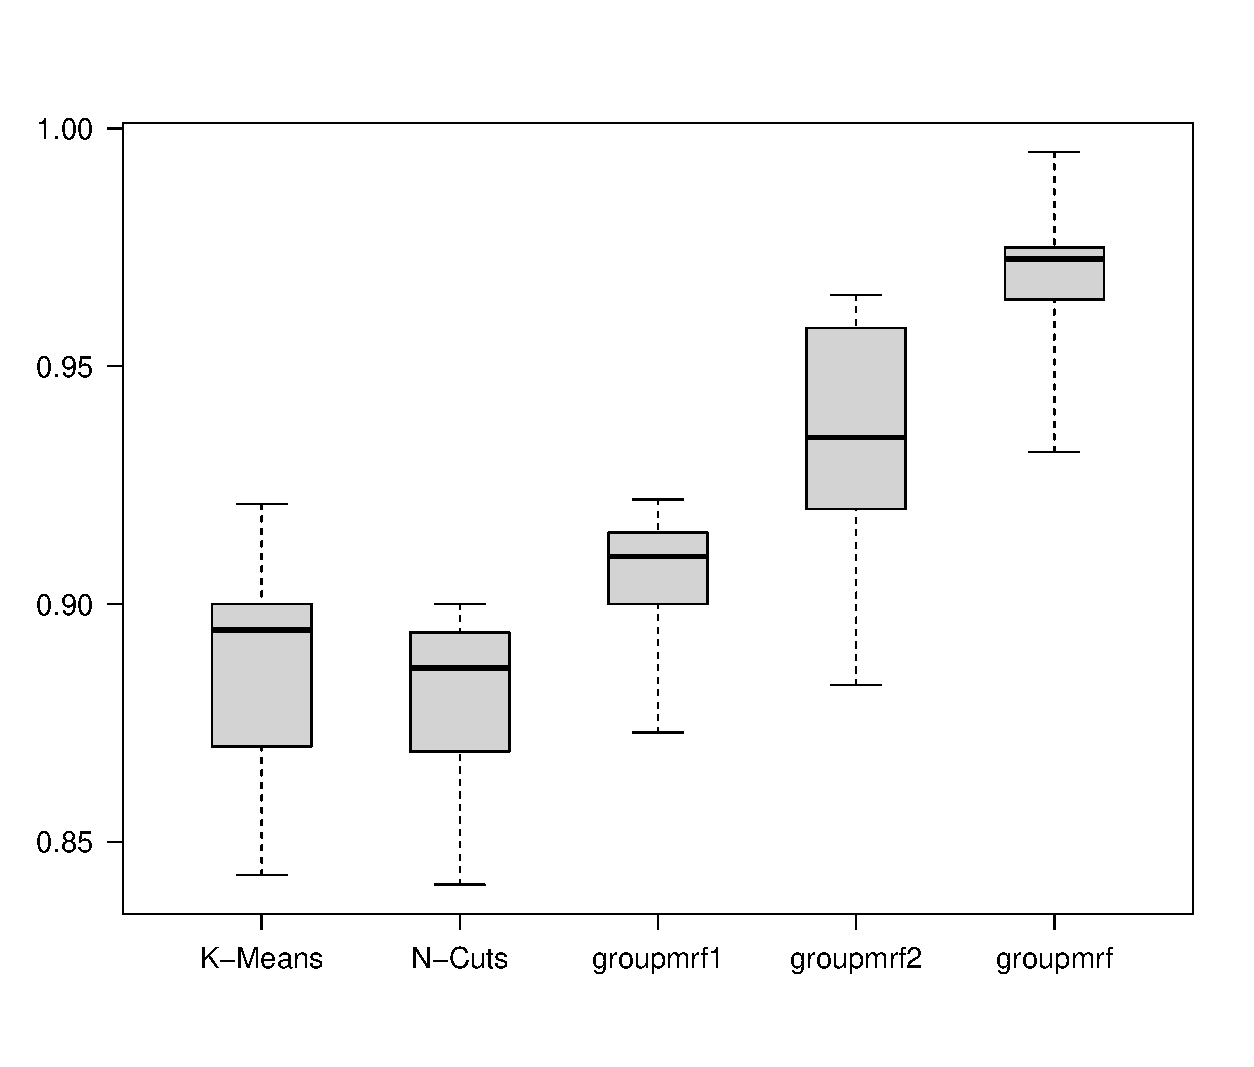
\includegraphics[width=0.5\textwidth]{figures/syn/rainplot}
  \caption{A box-Whisker plot of the Rand index value of all subjects label map
    for various methods. The bottom and top of the boxes are the $25$th and
    $75$th percentile, and the whiskers extends to the whole range of the data.}
  \label{fig:synboxplot}
\end{figure}

\subsection{Real Data}
\begin{figure*}[htb]
  \centering
  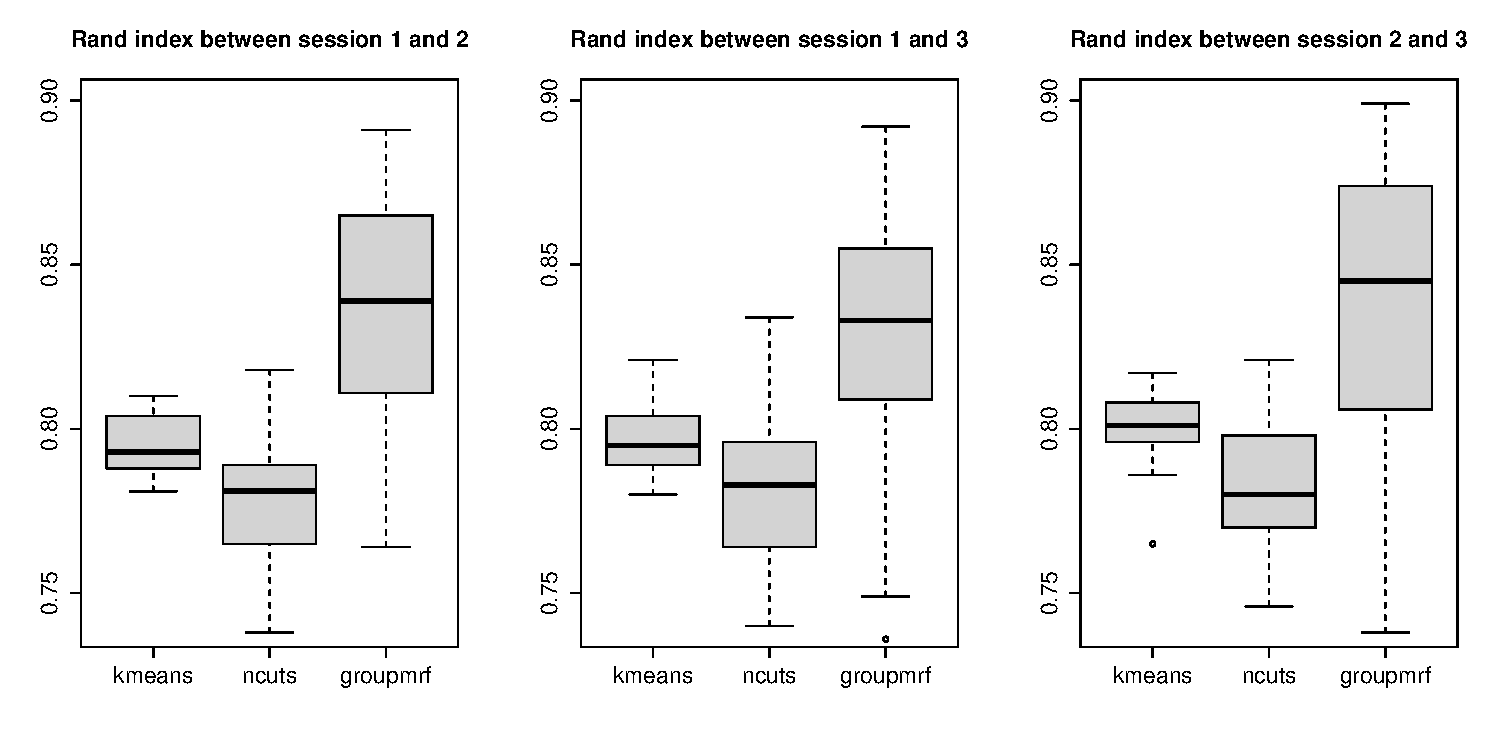
\includegraphics[width=0.9\textwidth]{rainlog/boxplot}
  \caption{}
  \label{fig:boxplot}
\end{figure*}

\appendix
\section{Plan for Experiments}
\cite{zuo2010reliable} is the group that first use New York test-retest
dataset. They use intraclass correlation (ICC) to compute the reliability at
each voxel. Their goal is to compare the ICC for different independent
components (ICs). Our goals are to show the hierarchical MRFs can get more
consistent maps compared to other methods. There are a few questions we need to
address:

1) What methods that the \textsf{groupmrf} can compare with?

2) What measurement to use? There are again a few options:

If we use ICC, we can compute the ICCs for each voxel, by using all three
sessions of all subjects. ICC is usually used on a continuous random variable,
so we can use the postior probability that we estimate from MC samples as the
r.v in ICC (I know it is not the best definition).  To be specific, following
\cite{zuo2010reliable}, we define $y_{ij}$ as the $j$th measurement made on the
$i$th subject. Here $j = 1, 2, 3$. We have the following decomposition

\[
y_{ij} = \mu + p_i + t_j + \epsilon_{ij}
\]


It is possible that we use the indicator variable of each MC sample as the
measurement, but that will add another level of variance and make things more
complicated. So we just use the posterior probability as a single summary of all
MC samples for each subject in each session.

For \textsf{groupmrf}, we will get a ICC map for each component. We will compute
the same map for other clustering method we want to compare with. Now we need to
compute a single number, i.e. a summary statistics from the ICC map, for the
purpose of comparison.

Instead, we can use \emph{Rand index} (RI), \emph{normalized Rand index} (NRI)
and \emph{normalized mutual information} (MNI) as the measurements for comparing
two clusterings. Rand index is applied on discrete segmentations of a dataset or
image. NRI is a normalize version of RI such that it has zero expectation. All 3
measures give single number for the similarity of two clusterings. We can do the
following steps

\begin{itemize}
\item We can show \textsf{groupmrf} has more consistent segmentations between
  subjects, but within session. We compute the pairwise similarity for all
  subject in one session, and average the RI values to get a mean RI. For
  other clustering methods, also compute the mean RI. Comparing these mean RI
  will show \textsf{groupmrf}'s advantage. The procedure can repeat for all 3
  sessions.

  This comparison will show the \textsf{groupmrf}'s advantage for sure.
  
\item We can show \textsf{groupmrf} gives more consistent segmentation across
  sessions. For each subject, we compute the similarity for each pair of 3
  sessions, and get ${3 \choose 2} = 3$ similarity numbers. Then I can average
  the numbers for all subjects and get a single similarity value. We do the
  same thing for other clustering methods.

  This comparison will probably show \textsf{groupmrf}'s advantage.

\item We can also compare the group map estimated from \textsf{groupmrf} and
  other methods. For our method, we have 3 group maps, and we compute the
  pairwise similarity for each pair of them. If other methods also has 3 group
  maps, we can compute the similarity also.
  
  Our method probably will not stand out in this experiment.
\end{itemize}


\bibliographystyle{model2-names}
\bibliography{/home/sci/weiliu/projects/centralref}
\end{document}
